\section{Thread-based Concurrency}
\label{sec:thread}
\subsection{Thread-based concurrency analysis} 

While concurrency is an important aspect defined by the UML State machine specification, especially hierarchical and concurrent state machines with \ti{doActivity}s for states, most of existing approaches do not take into account. This is non-trivial since concurrency is dynamic in UML state machine since the number of threads used for concurrency is non-deterministic.

For example, assuming that \ti{Idle} is the current active state of the ATM state machine in Fig. 
\ref{fig:example} and a \ti{verifyPIN} event is coming. 
The \ti{doActivity} behavior of \ti{Idle} \ti{doActivity(Idle)} (if has) is terminated, \ti{exit(Idle)} and the \ti{effect(t2)} (\ti{T2Effect}) are executed sequentially. 
These actions are run in a state machine main thread which reads incoming events from a "first in, first out" (FIFO) priority queue. 
Fig. \ref{fig:threading1} shows the activity diagram representing the concurrency of the state machine example when processing the \ti{verifyPIN} event, in which each activity partition represents a thread. 
The completion of \ti{effect(t2)} is followed by \ti{effect(t3)} and \ti{effect(t3)}, which are run concurrently since the transitions owning these effects outgo from a fork pseudo state. 
Two threads \ti{T3Run} and \ti{T4Run} associated with \ti{effect(t2)} and \ti{effect(t3)}, respectively, are created by \ti{FORK}.
The entry action \ti{entry(Verifying)} of \ti{Verifying} is executed following the termination of the two threads. 

After \ti{entry(Verifying)} completion, the UML specification says that \ti{doActivity(Verifying)}, \ti{entry(VerifyingCard)} and \ti{entry(VerifyingPIN)} should be concurrently executed, which is represented by a fork node, in which a \ti{Start} signal is sent to \ti{VerifyingDoRun} in order for commencing \ti{doActivity(Verifying)}. 
As the \ti{Verifying} state, the \ti{doActivity}s of the states \ti{VerifyingCard} and \ti{VerifyingPIN} are also concurrently started. 
Also, upon the completion of \ti{entry(VerifyingCard)} and \ti{entry(VerifyingPIN)}, the main thread completes the processing of the \ti{verifyPIN} event, reads next events from the queue or waits for next event occurrences.

\begin{figure}
	\centering
	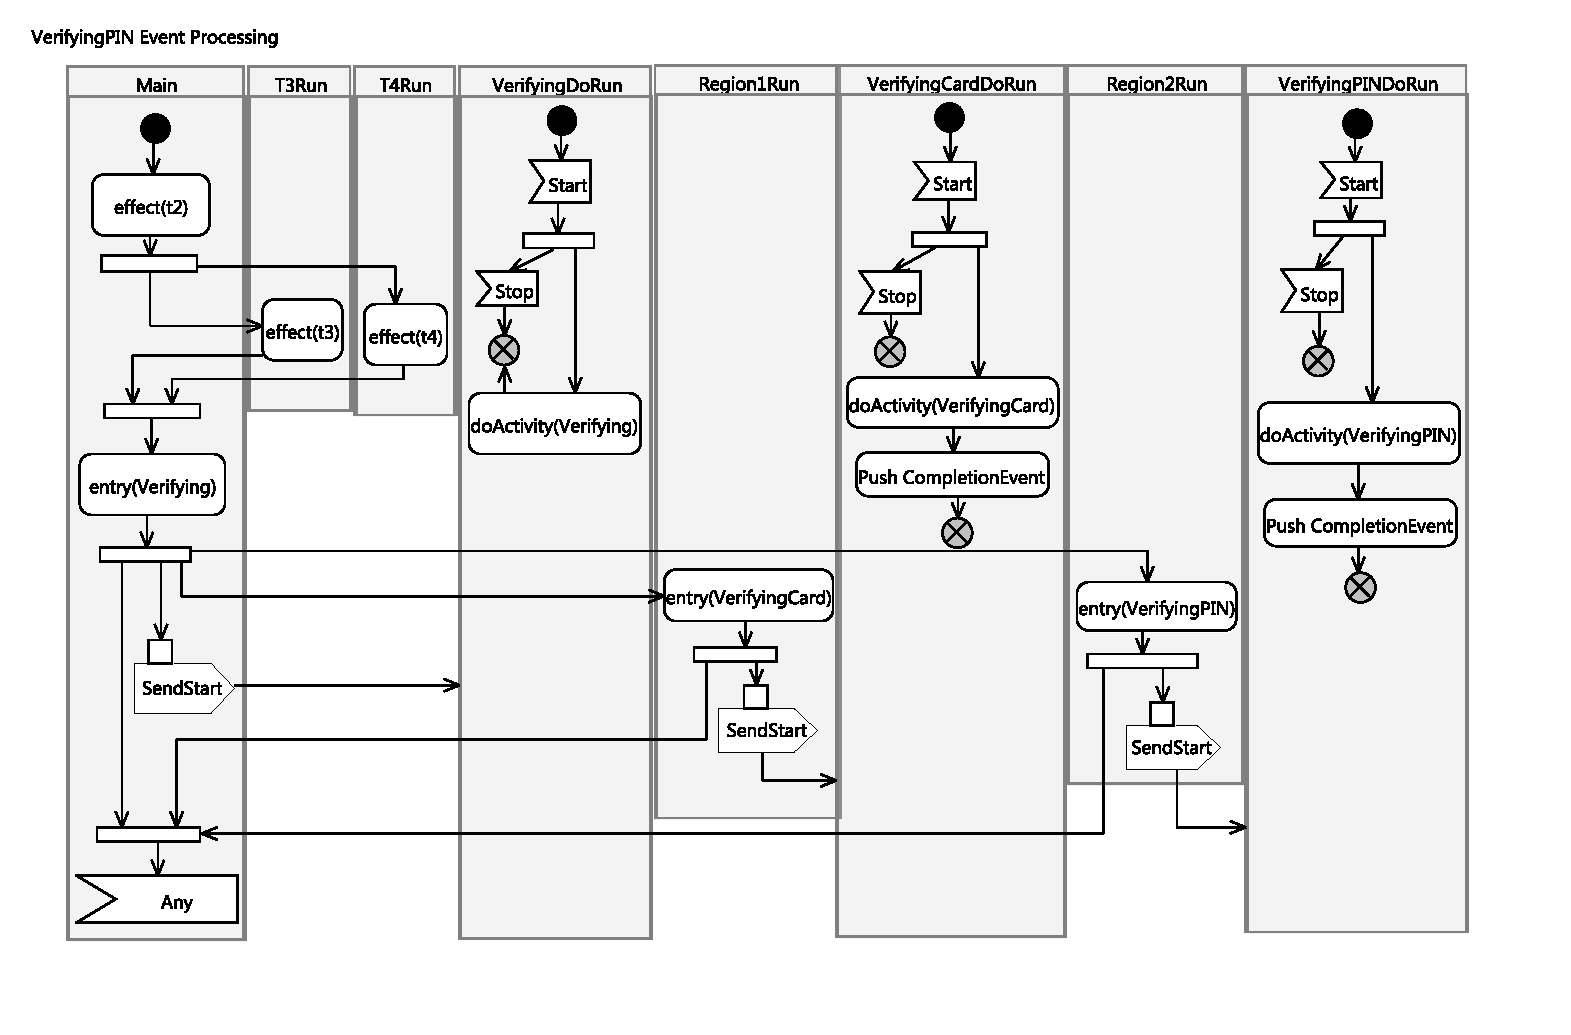
\includegraphics[clip, trim=1.0cm 1.6cm 1.6cm 1cm, width=1.03\columnwidth]{figures/ThreadingExample.pdf}
	\caption{Concurrency of the ATM when receiving the \ti{verifyingPIN} event} 
	\label{fig:threading1}
\end{figure}

If no event is coming, and \ti{doActivity(VerifyingCard)} and \ti{doActivity(VerifyingPIN)} are long actions (e.g. forever loops inside), the state machine remains its active configuration and three concurrent actions including \ti{CheckForEvents}, \ti{doActivity(VerifyingCard)}, and \ti{doActivity(VerifyingPIN)} are permanently run.

It is worth noting that the termination time of \ti{doActivity(VerifyingCard)} and \ti{doActivity(VerifyingPIN)} is non-deterministic. 
However, whenever one of those completes, a completion event associated with the state corresponding to the completed \ti{doActivity} is generated and pushed to the event queue. 
For illustration, assuming that \ti{doActivity(VerifyingCard)} terminates before \ti{doActivity(VerifyingPIN)}. 
As the activity diagram in Fig. \ref{fig:threading2}, the Main thread checks the \ti{CompletionEvent} upon the completion of \ti{doActivity(VerifyingCard)}. \ti{exit(VerifyingCard)} and \ti{effect(t5)} are then executed sequentially. If \ti{cardValid} is computed as true as the result of \ti{doActivity(VerifyingCard)} and \ti{exit(VerifyingCard)}, the Main thread simply executes \ti{effect(t6)} and \ti{entry(CardValid)} before waiting for other events.

In contrast, Main sends \ti{Stop} signals to stop \ti{doActivity(VerifyingPIN)} and \ti{doActivity(Verifying)}, executes exit actions, effects and entry actions in an appropriate order (see Fig. \ref{fig:threading2}) and waits for other events.

So far, we see that the number of concurrent actions is not constant but changes timely. 
Each action can either deterministically or non-deterministically terminate. 
In this sense, deterministic actions (DAs) prevent the Main thread from going to the waiting-for-event point. 
In other words, pending events in the queue are only read and processed once all deterministic actions complete. Therefore, we re-define the run-to-completion paradigm of UML state machine as following:
 
\begin{definition}
	Run-to-completion means that, in the absence of exceptions or asynchronous destruction of the context	class object or the state machine execution, a pending Event occurrence is dispatched only after the completion of all deterministic actions commenced by the processing of the current event. 
	At this point, a stable state configuration has been reached
\end{definition}

In the example, some of DAs are as followings: \ti{effect(t2)}, \ti{effect(t3)}, \ti{effect(t4)}, \ti{entry(Verifying)}, \ti{entry(VerifyingCard)}, \ti{entry(VerifyingPIN)} and non-deterministic actions (NDAs) as followings: \ti{doActivity(Verifying)}, \ti{doActivity(VerifyingCard)} and \ti{doActivity(VerifyingPIN)}.


\begin{figure}
	\centering
	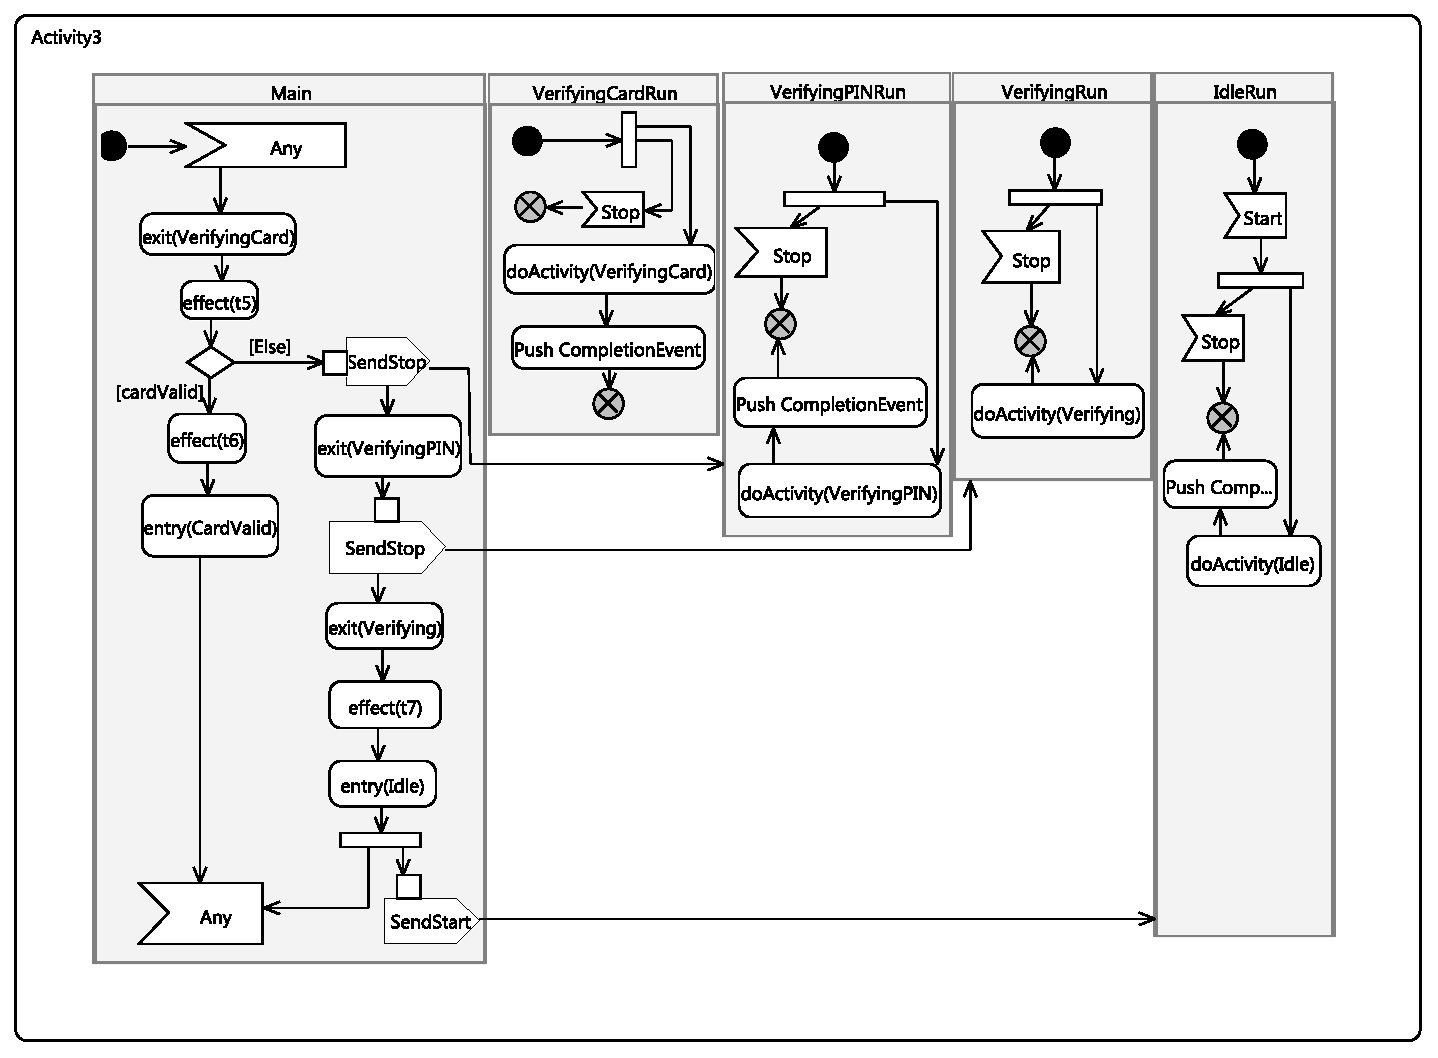
\includegraphics[clip, trim=1.5cm 1.6cm 1.6cm 1.2cm, width=1.03\columnwidth]{figures/ThreadingExample2.pdf}
	\caption{Concurrency of the ATM when \ti{doActivity} of \ti{VerifyingCard} completes before that of \ti{VerifyingPIN}}
	\label{fig:threading2}
\end{figure}

\subsection{Thread-based design of generated code}
Each NDA is run in parallel with the main thread which reads and dispatch events from the event queue. 
Each is associated with a thread which is initialized at the state machine initialization moment. 
The number of threads associated with NDAs is therefore equal to that of the NDAs.
The design of threads is based on the thread pool pattern, which initializes all threads at once, and the paradigm "wait-execute-wait". 
In the latter, a thread \tb{waits} for a signal to \tb{execute} its associated method and goes back to the \tb{wait} point if it receives a stop signal or its associated method completes. 
An NDA is one of the followings:
\begin{itemize}
	\item \ti{doActivity} of each state if has. The number of \ti{doActivity} $n_{do} = \#\{s \in V|\exists doActivity(s)\}$
	
	\item Sleep function associated with a \ti{TimeEvent} which counts ticks and emits a \ti{TimeEvent} once completes: $n_{te} = \#\{e \in E|\ti{e is a time event}\}$.
	
	\item Change detect function associated with a \ti{ChangeEvent} which observes a variable or a boolean expression and pushes an event to the queue if changes happen: $n_{che} = \#\{e \in E|\ti{e is a change event}\}$.
\end{itemize} 

Therefore, the concurrency has the number of initial threads $n_{threads} = n_{do} + n_{te} + n_{che}$ plus a main thread which reads events from the event queue, and sends start and stop signals to these initial threads. 

Now we consider spontaneous threads which are created by \ti{FORK} to run DAs, joined until and destroyed once DAs complete. The followings describe different types of DAs:

\begin{itemize}
	\item Actions executed when entering/exiting an orthogonal region, which can be: execute a chain of transition effects contained by the region before entering a stable sub-state or exiting the region completely.%: $n_{region threads} = \#\{r \in \mathcal{R}|ctner(r).kind=conc\}$
	
	\item Effects of transitions outgoing from a $fork$ and those incomings to a $join$.%: \\
	%$\mathcal{J} = \{v \in V|v.kind=join\}$ \\
	%$\mathcal{F} = \{v \in V|v.kind=fork\}$ \\
	%$$n_{FJ\_threads} = \sum_{v \in \mathcal{F}} {\#T_{outs}(v)} + \sum_{v \in \mathcal{J}} {\#T_{ins}(v)}$$.
\end{itemize}

The spontaneous threads follow a paradigm in which if a thread $parent$ creates a set of threads $children$, $parent$ must wait until $children$ complete their associate methods. These threads are created in one of the following cases:

\begin{itemize}
	\item Having multiple transitions outgoing from a \ti{fork}, for each transition effect, a thread is created by \ti{FORK}
	
	\item Entering a concurrent state $s$, after the execution of $entry(s)$, a thread is also created for each orthogonal region. 
	
	\item Exiting a concurrent state $s$, before the execution of $exit(s)$, a thread is also created for each region to exit the corresponding active sub-state. 
\end{itemize}

\subsection{Deadlock avoidance}
Deadlock is one of the main issues in designing multi-thread applications, in which two competing actions wait for the other to finish. In our case, 


\begin{comment}
\begin{tabular}{p{4.0cm}|p{4.0cm}}
Example code generated for doActivity  &  Option  2\\
\begin{lstlisting}[language=C++]
void doActivity(int stateId) {
  isStarts[stateId] = false;
  while(true) {
    mutex[stateId].lock();
    while(!isStarts[stateId]) {
      mutex[stateId].wait();
    }
    states[stateId].doActivity();
    isStarts[stateId] = false;
    mutex[stateId].unlock();
    if (!isStops[stateId]) {
      if (stateId == IDLE_ID || stateId == DISPENSEMONEY_ID ...) {
	    pushCompletionEvent(stateId);
	  }
    }
  }
}
	\end{lstlisting}&
	\begin{lstlisting}
	#include <stdio.h>
	
	int main()
	{
	printf("Hello world\n");
	}
	\end{lstlisting}
\end{tabular} 
\end{comment}
